\documentclass[11pt]{article}
\def\StudentVersion{}

\usepackage{../common}
\title{Game Playing}
\author{Alexander Rush}
\date{}
\def\LecStr{Alexander Rush}
\def\LecNum{2}
\def\LecTitle{Lecture Notes on Game Playing}
\def\LecDate{}

\begin{document}
\MakeScribeTop{}

\tikzstyle{utri}=[draw, regular polygon, regular polygon sides=3]
\tikzstyle{dtri}=[utri, shape border rotate=180]

\tableofcontents

\section{Introduction}

Game playing is one of the earliest pursuits of AI researchers. John McCarthy's students were already working on chess in 1959. Research into Chess culminated in 1997 when IBM's Deep Blue beat Gary Kasparov, becoming the first computer program to defeat the reining grand champion. Today you can download programs that are world-class at Chess even on standard hardware. 

However there are still many open challenges in adversarial search and game playing. XKCD is keeping score:

 
\begin{center}
  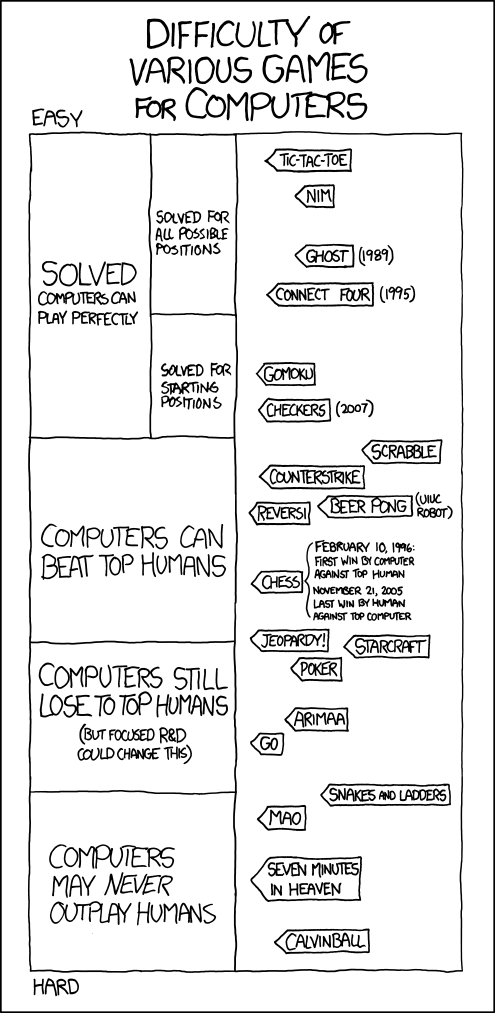
\includegraphics[height=13cm]{game_ais}
\end{center}

\noindent In this lecture we will use examples from Tic-Tac-Toe, later in the term we will talk about Jeopardy and StarCraft. Backgammon is also a particularly interesting example that we'll discuss briefly. If you're interested MIT has run a great IAP tournaments in the past focusing on Poker and StarCraft. There used to be a substantial reward for solving Go. However, Seven Minutes in Heaven is beyond the scope of this course.

\section{Game Playing}

We will be treating game playing as a search problem using a similar abstract specification. However there are several additional elements that we need to include.

\subsection{Game Model}

Game playing (GP) differs from search in that we will assume there are two game players Min and Max. Also unlike search where there was a cost associated with each action, in game playing there is a single \textbf{utility} that is only given at \textbf{terminal} (end) states. The Min player is aiming to minimize utility and the Max player to maximize utility. We assume that the game is \textbf{zero-sum}, i.e. at any terminal state the utility for Min and Max sums to zero, and \textbf{perfect information}, i.e. both players see the full state of the game.

 \air
\begin{center}
\begin{tabularx}{\linewidth}{llX}
  \toprule
  Name (AIMA) & Type & Description \\
  \midrule
\\
 State space & $\mcS$ & All possible states of the game, e.g. unique board positions \\\\
 Action space & $\mcA$& All possible actions of the game i.e. moves\\\\
 Actions&  $\msc{Actions}: \mcS \mapsto 2^\mcA$ & Actions are applicable at a given state, i.e. available moves. \\\\
 Transition model&  $\msc{Result}:  \mcS \times \mcA \mapsto \mcS $ &  Update the state after a move.  \\\\
 Initial state &  $S_0 \in \mcS$ & The starting state of the game.  \\\\
 \midrule \\
 Player& $\msc{Player}: \mcS \rightarrow \{\mathrm{Min}, \mathrm{Max}\}$ & Function indicating the current turn. \\\\
 Terminal test& $\msc{Terminal}: \mcS \mapsto \{0, 1\} $ & Predicate indicating if this state is terminal, i.e. is the game over. \\\\
 Utility & $\msc{Utility}: \mcS \rightarrow \reals$ & The utility at a (terminal) state. \\\\
 \bottomrule
\end{tabularx}
\end{center}

\subsection{Minimax}

The key challenge of adversarial search is that the agent does not control the decisions of its opponent. Therefore to behave rationally i.e. to minimize or maximize utility, the agent must model its opponents decisions. 

Generally we do this by assuming that the opponent will behave rationally as well, so if we are minimizing utility, we assume the opponent will act to maximize their utility. This leads to the Minimax formula for computing the utility of a nonterminal game state.

\[ \msc{Minimax}(s) = \begin{cases} 
  \censorm{\msc{Utility}(s)} & \mathrm{if\ } \msc{Terminal}(s)  \\
  \censorm{\max_{a \in \msc{Actions}(s)}  \msc{Minimax}(\msc{Result}(s, a))} & \mathrm{if\ } \msc{Player(s)} = \mathrm{Max}  \\
  \censorm{\min_{a \in \msc{Actions}(s) } \msc{Minimax}(\msc{Result}(s, a))} & \mathrm{if\ } \msc{Player(s)} = \mathrm{Min} \end{cases}\] 

We can expand this function into a data-structure known as a \textbf{game tree}. Each node in this tree represents a move by Max or Min. The triangles pointing up indicate that the node is maximizing over its children, and triangles pointing down indicate that the node is minimizing over its children.

\begin{center}
  \begin{tikzpicture}[sibling distance = 2cm]
    \Tree [ .\node[utri]{}; \edge node[auto=right] {Action 1};  [ .\node[dtri]{};  [  .\node[utri]{}; $\vdots$    ]   [ .\node[utri]{};  $\vdots$ ]
     ]  \edge node[auto=right] {Action 2}; [ .\node[dtri]{};   [ .\node[utri]{}; $\vdots$ ]  [ .\node[utri]{}; $\vdots$ ]  ]  \edge node[auto=left] {Action 3};  [ .\node[dtri]{};   [ .\node[utri]{}; $\vdots$ ]  [ .\node[utri]{}; $\vdots$ ]
    ] ]  
  \end{tikzpicture}
\end{center}



\subsection{Example: Tic-Tac-Toe}

Let's now consider one of the simplest zero-sum, perfect-information games, Tic-Tac-Toe. Consider the model for the following game state:


\begin{center}  
\begin{tabular}{c|c|c}
  O  &   &  \\
  \hline
  O  & X & X \\
  \hline
  X  & X & O
\end{tabular}
\end{center}

\begin{exercise}
  What is the model state at this stage of tic-tac-toe?
\end{exercise}
 \air
\begin{center}
\begin{tabularx}{\linewidth}{llX}
  \toprule
  Name & Type & Description \\
  \midrule
\\
 Actions&  \censor{$\msc{Actions}(s)= \{$ OTop, OTopRight$\}$} & \censor{There are currently two actions available to play.} \\\\
 Player& \censor{$\msc{Player}(s) = \mathrm{Min}$} & \censor{We will assume that O is minimizing utility and it is her  turn to play.} \\\\
 Terminal test& \censor{$\msc{Terminal}(s) = 0 $} & \censor{This is not a terminal state. We have yet to win or draw} \\\\
 Utility & \censor{$\msc{Utility}$} & \censor{The utility function at a terminal state will be 1 for X, -1 for O, 0 for a draw.} \\\\
 \bottomrule
\end{tabularx}
\end{center}

Next we can ask what is the utility that the Min player should assign to this state. We can do this by expanding out the recursive \textsc{Minimax} definition. This gives: 


\begin{eqnarray*} 
  \msc{Minimax}(s) = \min \{&& \max \{ \msc{Utility}(\msc{Result}( \msc{Result}(s, \mathrm{OTop})), \mathrm{XTopRight}) \}, \\
 & & \max \{ \msc{Utility}(\msc{Result}( \msc{Result}(s, \mathrm{OTopRight})), \mathrm{XTop}) \} \} 
\end{eqnarray*}

\noindent Since either way O plays, it leads to an X win, this utility of this state is $1$. 

\begin{exercise}
 Can we also write the same calculation as a game tree?
\end{exercise}


\ifthenelse{\isundefined{\StudentVersion}}{
\censor
\begin{center}
  \begin{tikzpicture}[sibling distance = 2cm]
    \Tree [ .\node[dtri]{}; \edge node[auto=right] {OTop}; [  .\node[utri]{}; \edge node[auto=left] {XTopRight}; 1 ] \edge node[auto=left] {OTopRight}; [ .\node[utri]{}; \edge node[auto=left] {XTop}; 1
    ] ]
  \end{tikzpicture}
\end{center}

} {
\censor{}
\vspace{5cm}
} 

Now let's consider a slightly more interesting position from X's perspective

\begin{center}  
\begin{tabular}{c|c|c}
  O  &   &  \\
  \hline
  X  & O &  \\
  \hline
  X  & O & X
\end{tabular}
\end{center}


\begin{exercise}
 Let's write the same calculation as a game tree.
\end{exercise}

\ifthenelse{\isundefined{\StudentVersion}}{
\censor{}

\begin{center}
\scalebox{0.8}{\begin{tikzpicture}[sibling distance = 2cm]
    \Tree [ .\node[utri]{}; \edge node[auto=right] {XTop};  [ .\node[dtri]{}; \edge node[auto=right, yshift=0.5cm] {OTopRight}; [  .\node[utri]{}; \edge node[auto=left] {XRight}; 0 ] \edge node[auto=left] {ORight}; [ .\node[utri]{}; \edge node[auto=left] {XTopRight}; 0
    ] ] \edge node[auto=right] {XTopRight}; [ .\node[dtri]{}; \edge node[auto=right] {OTop};  -1 \edge node[auto=left] {ORight}; [ .\node[utri]{}; \edge node[auto=left] {XTop}; 0 ] 
     ]  \edge node[auto=left] {XRight}; [ .\node[dtri]{}; \edge node[auto=right] {OTop};  -1 \edge node[auto=left] {OTopRight}; [ .\node[utri]{}; \edge node[auto=left] {XTop}; 0 ] 
    ] ]  
  \end{tikzpicture}}
\end{center}
} {

\censor{}
\vspace{10cm}
}

The max player (X) can at best play for a draw here. 
Clearly the right play is XTop which gives the utility of 0. 

Note though that for these problems we are only considering a branching factor of at most 3, and a depth of 2. In practice the tree grows very large, very quickly.
AIMA has a nice graphic showing a partial  expansion of a game tree for tic-tac-toe from scratch. 

\begin{center}
  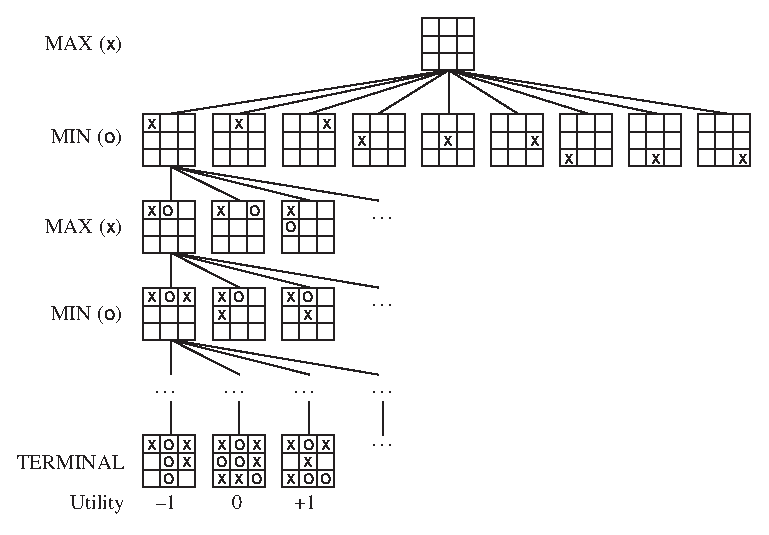
\includegraphics{tictactoe}
\end{center}

\section{Search for Game Playing}

As with standard search, we have to decide how to 
enumerate possible game states in order to find a path to take. We do this by implementing search over the Minimax game tree. 

In particular, we utilize uninformed depth-first tree search where are terminal states are goal states. 
\begin{exercise}
  Why do we not need to use graph search for games? Why not use uniform-cost search?
\end{exercise}

\censor{}


In this situation, DFS has clear advantages over BFS in terms of memory-efficiency. Because of the nature of game playing, we do not have to worry about maintaining the costly expand list. 
Note also that instead of explicitly using a stack, we can implement DFS using recursion. Each recursive call to \textsc{Minimax} simulates a pushing and popping from the stack. This leads to a very simple implementation of Minimax Search. 
\air

% The minimax algorithm can be seen as a special case of DFS. For a game with $m$ levels to the furthest terminal state it requires $O(b^m)$ steps to compute this function. Of course this is   

\begin{algorithm}[h]
\begin{algorithmic}[1]
  \Procedure{Minimax}{$s$}

  \If{$\msc{Terminal}(s)$}
  \Return{$\msc{Utility}(s)$}
  \ElsIf{$\msc{Player}(s) = \mathrm{Max}$}
  \State{$v \gets \censorm{-\infty}$}
  \For{$a \in \msc{Actions}(s)$}
  \State{\censor{$v \gets \max\{v, \msc{Minimax}(\msc{Result}(s, a))\}$}}
  \EndFor{}
  \ElsIf{$\msc{Player}(s) = \mathrm{Min}$}
  \State{$v \gets \censorm{\infty}$}
  \For{$a \in \msc{Actions}(s)$}
  \State{\censor{$v \gets \min\{v, \msc{Minimax}(\msc{Result}(s, a))\}$}}
  \EndFor{}
  \EndIf{}
  \State{\Return{$v$}}
  \EndProcedure{}
\end{algorithmic}
\end{algorithm}


% \noindent The pseudo-code here is basically a direct implementation of the mathematical definition of \textsc{Minimax}. However, the recursive implementation means we search deeper before searching broader.

\begin{exercise}
  What is the space and time complexity of this algorithm?
\end{exercise}

\censor{
  Again let $m$ be the depth of the deepest terminal state and $b$ be
  the max branching factor. This algorithm need to enumerate each
  possible state to this point giving a run-time of $O(b^m)$. However
  at any one time, it only needs memory for all actions at each state
  along the path to the deepest goal. This gives a memory complexity
  of $O(bm)$.}


\subsection{Alpha-Beta Pruning}

We can further speed up game-playing search by exploiting some properties about the game tree.  One nice property of the $\max$ ($\min$) operator, is that if we know after seeing $i$ elements of the set that known of the future elements will be greater (less) then it is not necessary to compute these values at all. We can therefore \textbf{short circuit} the computation and return.


Consider the following example:

\vspace{1cm}


  \begin{tikzpicture}[sibling distance = 2cm]
    \Tree [ .\node[utri]{};   
    [ .\node[dtri]{};  [  .\node[utri]{}; 5    ]   [ .\node[utri]{};  10 ] ]  
    [ .\node[dtri]{};   [ .\node[utri]{}; 3 ]  [ .\node[utri]{}; 12 ]     [ .\node[utri]{}; -1 ]  [ .\node[utri]{}; 1 ]
    ] ]  
  \end{tikzpicture}


  \begin{exercise}
    Go through this example and calculate the value of each state of the game tree top-down, left-to-right.
    What is the minimax value of the top state?
  \end{exercise}
\censor{}

  \begin{exercise}
    If instead of $-1$ the utility was $-1000$, would anything change? What if instead $5$ was equal to $2$?
  \end{exercise}
\censor{}

What happened in this case was that the already computed value $5$ already dominated the value of $3$ in the min. Since $3$ is already lower than $5$ there is no need to keep on calculating the rest of the values. 

\textbf{Alpha-beta pruning} exploits this idea to speed up Minimax computation without changing the final result. Formally this comes up when where there is a min embedded inside a max:

\[ \max\{ \alpha, \ldots,  \min\{\ldots, v, \ldots, v' \} \}\]
  
\noindent Let's say we have already computed the value of $\alpha$ and $v$, but are deciding whether to compute the rest of the min including $v'$. Consider the two cases:

\begin{enumerate}
\item  $v \geq \alpha$; the inner $\min$ may end with a value higher than $\alpha$ 
\item  $v \leq \alpha$; the inner $\min$ will never affect the outer max, so calculating the value of $v'$ tells us no new information. 
\end{enumerate}

In our examples the \textbf{alpha} value was $\alpha = 5$ and $v=3$. Since we are in the second case there is no need to keep calculating values.

We can generalize this idea to any of the outer max's:

\[ \max\{ \ldots, \alpha, \ldots, \min\{ \max\{\ldots \min\{\ldots, v, \ldots, v' \} \}\} , \ldots\}\]

If there is a future value $v'$ with $v' \leq v$ it may be selected by the inner $\min$. However we know $v' < v \leq \alpha$ so it will not be selected by the outer $\max$. The bigger $\alpha$ we have, the more likely we can apply this pruning, so we maintain the largest $\alpha$ seen at ancestor $\max$ node. 

We can also reverse this trick for $\min$ nodes by maintaining the smallest $\beta$ value:

\[ \censorm{\min\{ \ldots, \beta, \ldots, \max\{ \min\{\ldots \min\{\ldots, v, \ldots, v' \} \}\} , \ldots\} }\]

The modified Minimax search algorithm is shown below.
The upside of this method is that it yields a significant speed-up in practice with very minimal bookkeeping and no effect on the result. A rare combination.

\begin{algorithm}
\begin{algorithmic}[1]
  \Require{$\alpha$ is highest value of ancestor max-node, 
    $\beta$ is lowest value of ancestor min-node}
  \Procedure{AlphaBetaMinimax}{$s$, $\alpha$, $\beta$}

  \If{$\msc{Terminal}(s) = 1$}
  \Return{$\msc{Utility}(s)$}
  \ElsIf{$\msc{Player}(s) = $ Max}
  \State{$v \gets $\censor{}}
  \For{$a \in \msc{Actions}(s)$}
  \State{$v \gets$ \censorm{$\max\{v, \msc{AlphaBetaMinimax}(\msc{Result}(s, a), \alpha, \beta)\}$}}
  \If{$v \geq \beta$}
  \Return{$v$}
  \EndIf{}
  \State{$\alpha \gets \max\{\alpha, v\}$}
  \EndFor{}
  \ElsIf{$\msc{Player}(s) = $Min}
  \State{$v \gets $\censor{}}
  \For{$a \in \msc{Actions}(s)$}
  \State{$v \gets$ \censorm{$\min\{v, \msc{AlphaBetaMinimax}(\msc{Result}(s, a), \alpha, \beta)\}$}}
  
  \If{\censorm{$v \leq \alpha$}}
  \Return{$v$}
  \EndIf{}
  \State{\censorm{$\beta \gets \min\{\beta, v\}$}}
  \EndFor{}
  \EndIf{}
  \State{\Return{$v$}}
  \EndProcedure{}
\end{algorithmic}
\end{algorithm}



\subsection{Real-Time Decisions}

While alpha-beta pruning does give a speed-up, most games are still much too large to compute \textsc{Minimax} in practice. Chess for instance has a average branching factor of 35 and an average depth of 40 (apparently there was a 277 move game once). Of course $O(35^{40})$ is cartoonishly large:

\[ 57905761067641178540192733082440108773880638182163238525390625\] 

In practice game playing systems use either a depth-limited search approach or an iterative deepening approach. For both, a depth limit is selected and search is cutoff at this depth. 

\[ \msc{H-Minimax}(s, d) = \begin{cases} 
  \msc{Utility}(s) & \mathrm{if\ } \msc{Terminal}(s)  \\
  h(s) & \mathrm{if\ } d > \mathrm{limit}   \\
  \max_{a \in \msc{Actions}(s) } \msc{H-Minimax}(\msc{Result}(s, a), d+1) & \mathrm{if\ } \msc{Player(s)} = \mathrm{Max}  \\
  \min_{a \in \msc{Actions}(s) } \msc{H-Minimax}(\msc{Result}(s, a), d+1) & \mathrm{if\ } \msc{Player(s)} = \mathrm{Min} \end{cases}\] 

However, unlike in the standard search setup, GP only receives a score when it reaches a terminal state. To handle depth limited cases, we need a function $h: \mcS \mapsto \reals$ to award a heuristic utility to the state. As with general search, coming up with good game-specific heuristics is a very challenging problem but crucial to the construction of effective and practical GP agents.  

\subsection{Heuristics}

Generally game playing heuristics estimate how good a position is for each player. Note that unlike search heuristics we will not make any attempt to maintain admissibility or consistency here, although similar conditions do exist.

Perhaps the simplest heuristic is the value system taught to beginners learning to play chess. This system simply assigns value to the \textbf{material remaining} on the board. 
\air

\centerline{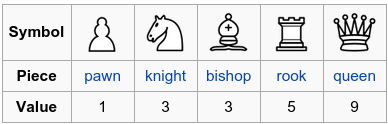
\includegraphics[width=8cm]{chessvalues1}}
\air

However, note that because this is just an approximation and ignores so much of the other complications of chess, there have been many, many other heuristics for this problem. (Wikipedia is amazing.) I am not a chess player, but it is pretty remarkable to me that not even the relative values of bishop and knight are consistent.

\centerline{ 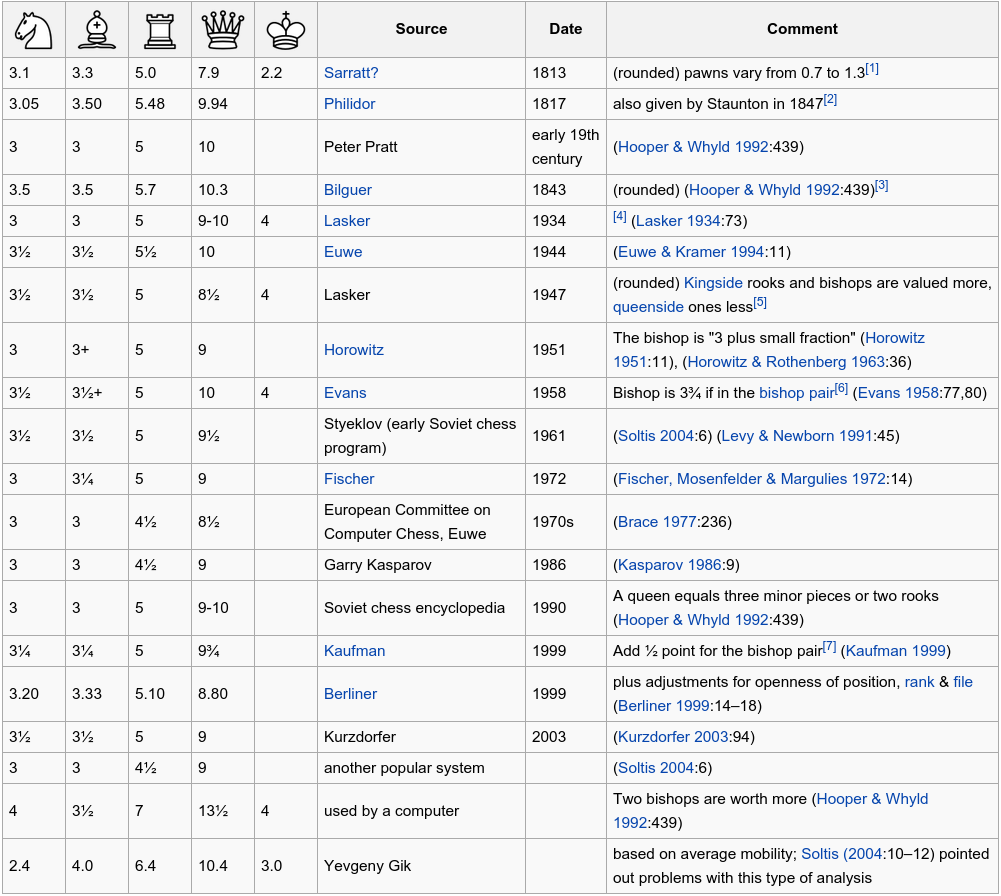
\includegraphics[width=16cm]{chess_value}}
\vspace{1cm}

Another method that is used is brute force calculation of certain positions. In chess this often means utilizing an end-game solver to play out the results of a large set of standard positions (such as a kings and pawns ending) . Given that each extra depth is a multiplicative cost, having an endgame database can turn a failed search into a successful one.





\subsection{Expecti-Max}

So far we have consider only deterministic games with perfect information. We will end by discussing games like Backgammon, which have perfect information but incorporates randomness. Each turn in backgammon consists of two steps:

\begin{itemize}
\item Roll two dies
\item Select checkers to move based on dice values. 
\end{itemize}

Our focus will be on the question of how to model our opponent Min's action. Since we don't know what value they will roll, we could be pessimistic and assume that they get the best possible roll ($\min$ over rolls) or optimistic assume they get the worst possible roll ($\max$ over rolls). 


Instead, we will directly model the randomness of the roll. We treat the dice roll as a third play Exp and the value of the dice as an action $a$. Given the state of the world $s$, we say the probability of Exp taking action $a$ is given as $P(a | s)$. 

In the case of Backgammon, there are $36$ possible actions corresponding to each pair of dice rolls, each with probability $\frac{1}{36}$. The turn order then alternates: Exp, Min, Exp, Max, Exp, Min, ...
Once we explicitly incorporate the last roll into the state $s$, the moves of Max and Min become deterministic.  


Why do we call this third player Exp? Well, similar to Max and Min, nodes in the game tree associated with Exp will take the \textbf{expectation} over children nodes. Define the expectation of a function $f$ with respect to a random variable $x$ as:

\[\mathbb{E}_{x|y}[f(x)] = \sum_{x} p(x|y)f(x) \]

In the case of the utility of a state, this gives us a method for computing the expected utility of an Exp state.

% In other games the randomness may take various other forms. 


% consider the case of a game with randomness. We model randomness as a third player Exp. Assume that at random states there is a probability distribution $p(a | s)$ of selecting an action $a$. Define expectation of 

\[ \mathbb{E}_{a|s}[\msc{Utility}(\msc{Result}(s, a))]= \sum_{a \in \msc{Actions}(s) } p(a | s) \msc{Utility}(\msc{Result}(s, a))  \]  

This formula can then be directly plugged into minimax, to yield an algorithm known as expectimax

\[ \msc{E-Minimax}(s) = \begin{cases} 
  \censorm{\msc{Utility}(s)} & \mathrm{if\ } \msc{Terminal}(s)  \\
  \censorm{\max_{a \in \msc{Actions}(s) } \msc{E-Minimax}(\msc{Result}(s, a))} & \mathrm{if\ } \msc{Player(s)} = \mathrm{Max}  \\
  \censorm{\min_{a \in \msc{Actions}(s) } \msc{E-Minimax}(\msc{Result}(s, a))} & \mathrm{if\ } \msc{Player(s)} = \mathrm{Min} \\ 
  \censorm{\sum_{a \in \msc{Actions}(s) } p(a | s) \msc{E-Minimax}(\msc{Result}(s, a))} & \mathrm{if\ } \msc{Player(s)} = \mathrm{Exp} \end{cases}\] 


\end{document}